\section{Umsetzung des Prototypen emoTrix}
In diesem Abschnitt wird die Umsetzung des Prototyps für die mobile Applikation emoTrix beschrieben. Dabei werden neben dem Programmcode auch aufgetretene Probleme beschrieben.
\subsection{Umsetzung der Backendlogik}
Dieses Kapitel thematisiert die Implementierung der Klassen \textit{Sensor}, \textit{CausalityRule} und \textit{Decider}, die das Backend der App ausmachen. Die wesentlichen Funktionen und Eigenschaften sind hierbei in Codeauschnitte abgebildet.
\subsubsection{Sensor-Klasse}
\subsubsectionauthor{Torben Brenner}
Wie im Konzept beschrieben besteht das Backend der Anwendung aus den Klassen \textit{Decider, CausalityRule} und der Abstrakten Klasse \textit{Sensor}. Im folgenden wird die Umsetzung der einzelnen Klassen beschrieben.\newline
Die Klasse \textit{Sensor} wurde als Abstrakte Klasse umgesetzt. Dies ermöglicht es dem Entwickler, für jeden Test eine Klasse zu implementieren die von der Architektur verstanden wird und in der er die im Test ermittelten Daten auswerten kann. Die Implementation der \textit{Sensor} Klasse sieht folgendermaßen aus: \newline
\begin{lstlisting}[caption={abstrakte Klasse Sensor},language=JavaScript]
export abstract class Sensor{

	observable: Observable<string>;
	sensorObserver: Observer<string>;

	constructor(public decider: Decider){
		this.observable = Observable.create(observer => {
			this.sensorObserver = observer;
		});
	};

	// this forces the specific sensor evaluators to implement this method
	abstract mapper(data: any): IndicatorScore[]; 

	onSensorData(data: any) {
		let indicatorScores = this.mapper(data)
		this.decider.addIndicatorScores(indicatorScores);
	}

}
\end{lstlisting}
Der Konstruktor der Klasse empfängt eine Instanz der Klasse \textit{Decider}, die wie im Konzept beschrieben ein Singleton ist. Die Funktion \textit{onSensorData} wird von den Subklassen aufgerufen, sobald Daten empfangen wurden und stellt die Logik der Sensor Klasse dar. Zuerst wird bei Empfang der Daten, das von erbenden Klassen definierte \textit{Mapping} auf die Daten ausgeführt. Danach werden die Daten dem \textit{Decider} hinzugefügt, welcher diese dann im späteren Verlauf verarbeiten kann(Vgl. \ref{img:Ablauf Erstellung Indicatorscores}). Durch das Schlüsselwort \textit{abstract} wird bei der Funktion \textit{mapper} gekennzeichnet, dass dieser von den erbenden Klassen implementiert werden soll. Die Abstrakte Klasse definiert in diesem Fall nur, dass der Mapper aus den Daten des Sensors eine Liste von \textit{IndicatorScores} erzeugen muss. Ein \textit{IndicatorScores} besteht dabei aus einem \textit{indicator} und einem \textit{score}. Der Score ist als nummerischer Wert definiert und für die Indicator wurde ein eigener Typ definiert. Dieser Typ ermöglicht es, eine einfache Prüfung der Werte gegenüber dem Typ String und bestimmten Werten durchzuführen. Erlaubte Werte für den Typ Indicator sind zum Beispiel: \textit{``stress''} oder \textit{``angryIndicator''}.\newline
Wie im Konzept beschrieben, verwaltet die Klasse \textit{Decider} alle \textit{IndicatorScores}. Um sicherzustellen, dass die Daten nach Zeitpunkt sortiert gespeichert werden, ermittelt die Methode \textit{addIndicatorScores} erst einen Zeitpunkt und speichert danach die Daten in einer List von Objekten, welche den Zeitpunkt und die dazu gehörige Liste von \textit{IndicatorScores} enthalten. Dadurch können Sensoren die \textit{IndicatorScores} einfach dieser Liste hinzufügen, ohne Gefahr zu laufen, sich gegenseitig zu überschreiben.\newline
Um eine Kommunikation der speziellen Sensoren mit den implementierenden Seiten zu erlauben, wurde der Sensor Klasse ein \textit{Observable} hinzugefügt. Dieses ermöglicht es der Seite sich als \textit{Subscriber} einzutragen. Ein \textit{Subscriber} erhält jedes mal eine Mitteilung, wenn die \textit{next} Funktion des Observers aufgerufen wird. Der Observer wird im Konstruktor aus dem \textit{Observable} erzeugt. Subscriber müssen eine Methode implementieren, in der Sie die Nachrichten des \textit{Observable} verarbeiten. Diese Kommunikation ist Beispielsweise in der Implementation des \textit{FaceSensor} zu sehen.
\subsubsection{CausalityRule-Klasse}
\subsubsectionauthor{Torben Brenner}
Um die Auswertung der Daten zu ermöglichen, greift die Klasse \textit{Decider} außerdem auf eine Liste von Kausalitätsregeln zu. Diese können mit der Klasse \textit{CausalityRule} definiert werden.
Der Konstruktor dieser Klasse nimmt zwei Parameter entgegen. Der Parameter \textit{condition} repräsentiert eine Bedingung, welche eintreten muss sodass die Kausalitätsregel angewandt wird. Die Bedingung wurde innerhalb der Anwendung durch einen Typ umgesetzt. Der Typ prüft dabei auf eine Funktion, die entweder einen oder zwei \textit{indicator} als Parameter entgegennimmt, und als Rückgabewert wahr oder falsch zurückgibt.\newline \newline \newline
\begin{lstlisting}[caption={Typ condition}, language=JavaScript]
	type Condition = (indicatorA: IndicatorScore, indicatorB?: IndicatorScore) => boolean;
\end{lstlisting}
Das bedeutet, dass die Bedingung vom Entwickler frei über die \textit{IndicatorScores} definiert werden kann. Der zweite Parameter der Anwendung repräsentiert die Auswirkungen der Kausalitätsregel beim eintreffen der Bedingung. Um diesen Parameter zu definieren wurde ebenfalls ein neuer Typ angelegt. Dieser prüft auf Funktionen, die sowohl eine Liste von \textit{EmotionScores} als auch eine Liste von \textit{IndicatorScores} entgegen nehmen. Außerdem müssen diese Funktionen eine Liste von \textit{EmotionScores} zurückgeben. Das bedeutet, dass in Funktionen dieser Art irgendeine Manipulation der \textit{EmotionScores} stattfinden muss. Die \textit{IndicatorScores} werden benötigt, um eine Veränderung der \textit{EmotionScores} abhängig von ihnen zu ermöglichen. Der zweite Parameter der Kausalitätsregel ist eine Liste solcher Funktionen. Mit diesen beiden Funktionen kann nun in der Klasse \textit{CausalityRule} eine neue Funktion definiert werden, die prüft ob eine Bedingung eingetroffen ist und in diesem Fall, alle Auswirkungen der Regel ausführt. \newline
\begin{lstlisting}[caption={execute Funktion der Klasse CausalityRule},language=JavaScript]

public execute(data : Array<EmotionScore>, indicatorScores: IndicatorScore[]) {
	indicatorScores.forEach((indicatorScore) =>{
		if(this.condition(indicatorScore)){
			this.effects.forEach((effect) => {
				data = effect(data);
			})
		}});
		return data;
	}
}

\end{lstlisting}
Diese Funktion kann nun von der Klasse \textit{Decider} ausgeführt werden. \newpage
\subsubsection{Decider-Klasse}
\subsubsectionauthor{Lukas Seemann}
Im folgenden Abschnitt wird die Implementierung der wichtigsten Funktionen der \textit{Decider} Klasse aufgezeigt und beschrieben. \newline
\begin{lstlisting}[caption={Atrribute der Decider-Klasse}, language=JavaScript]
@Injectable()
export class Decider {

data: Array<{timestamp: number, indicatorScores: IndicatorScore[]}> = [];
resultData: Array<{timestamp: number, emotionScores: EmotionScore[]}> = [];
causalityRules: Array<CausalityRule> = CRarray;

	...
}
\end{lstlisting}
In Listing ? sind die Attribute der \textit{Decider}-Klasse, wie sie auch schon in der Architektur eingeführt worden abgebildet. Das Array \textit{data} in Zeile 4 enthält IndicatorScores mit dem Zeitpunkt in Millisekunden, an dem diese Scores hinzugefügt wurden. Das Hinzufügen ist über die Mapper der einzelnen Sensoren geschehen, die die addIndicatorScore-Funktion des Deciders aufrufen.\newline
In Zeile 5 wird das \textit{resultData}-Array initialisiert. Anhand der vorhandenen IndicatorScores im \textit{data}-Array werden mithilfe der Kausalitätsregeln für alle 10 Sekunden in EmotionScores umgewandelt. Wie dies umgesetzt ist, ist in der decide-Funktion zu sehen. \newline
In Zeile 6 wird das Array der \textit{CausalityRules} über eine Konstante \textit{CRArray} initialisiert. Dieses konstante Array wird in Kapitel 4.3.2 genauer beschrieben. \newline \newline
\begin{lstlisting}[caption={decide-Funktion der Decider-Klasse}, language=JavaScript]
public decide(){
	let start: number = this.findRange().start;
	let end: number = this.findRange().end;
	for(var i:number = start; i<=end; i= i+ 10000){
		var j: number = i + 9999;
		this.assumeEmotion(i, j);
	} 
}
\end{lstlisting}
Die decide-Funktion ist in Listing 5 abgebildet. Mithilfe der internen findRange-Funktionen werden in den Zeilen 2 und 3 die minimale beziehungsweise maximale \textit{timestamp} des \textit{data}-Array bestimmt. So hat man der ersten und letzten Zeitpunkt (in Millisekunden) gefunden, zu dem IndicatorScores durch die einzelnen Test hinzugefügt wurden. \newline
Mithilfe einer for-Schleife (Zeile 4) wird anschließend in 10 Sekunden-Schritten über den durch \textit{start} und \textit{end} festgelegten Bereich iteriert. Dabei wird in der for-Schleife in Zeile eine Hilfsvariable \textit{j} eingeführt, die mit dem Iterator \textit{i} plus 9999 Millisekunden initialisiert wird. Mithilfe von \textit{i} und \textit{j} wird also in jedem Iterationschritt ein Intervall von 10 Sekunden festgelegt. Auf dieses Intervall wird in Zeile 6 die assumeEmotion-Funktion angewendet. \newline
\begin{lstlisting}[caption={assumeEmotion-Funktion der Decider-Klasse}, language=JavaScript]
private assumeEmotion(start: number, end: number){
	let currentIndicators = this.data.filter(e => e.timestamp >= start &&   e.timestamp <= end)
	var emotionScores: Array<EmotionScore> = this.executeCausalityRules(currentIndicators);
	this.resultData.push({ timestamp: start, emotionScores: emotionScores});
}
\end{lstlisting}
Listing 6 zeigt den Aufbau der assumeEmotion-Funktion, die einen \textit{start} und ein \textit{end} als Parameter erhält. Anhand dieser Zahlen wird anfangs in Zeile 2 das \textit{data}-Array gefiltert. Hierbei werden alle Einträge in eine Variable \textit{currentIndicators} geschrieben, die mit ihrer \textit{timestamp} zwischen \textit{start} und \textit{end} liegen. \newline
In Zeile 3 wird dann eine neue Variable \textit{emotionScores} intialisiert, die als Wert das Ergebnis der executeCausalityRules-Funktion angewandt auf die \textit{currentIndicators} erhält. Die Implementierung dieser Funktion, die EmotionScores zurückliefert, ist in Listing 7 zu sehen. In Zeile 4 von Listing 6 werden dann diese Emotionscores mit der \textit{start}-Timestamp zum \textit{resultData}-Array hinzugefügt. \newline 
\begin{lstlisting}[caption={executeCausalityRules-Funktion der Decider-Klasse}, language=JavaScript]
private executeCausalityRules(data: Array<{timestamp: number, indicatorScores: IndicatorScore[]}>){   
	var emotionScores: EmotionScore[] = [];
	emotions.forEach(emotion => {
		var emotionScore : EmotionScore = {emotion, score: 0};
		emotionScores.push(emotionScore);
	});
	data.forEach((e) =>  { 
		this.causalityRules.forEach((causalityRule) => {
			emotionScores = causalityRule.execute(emotionScores, e.indicatorScores)  ;
		})}
	)
	return emotionScores;
}
\end{lstlisting}
Die executeCausalityRules-Funktion erhält als Input ein Array von \textit{timestamp}-\textit{IndicatorScores}-Kombinationen. Zunächst wird in Zeile 2 ein leeres EmotionScore-Array initialisiert. In den Zeilen 3 bis 6 wird dieses dann befüllt, indem für jede vorhandene Emotion (angry, happy, sad, suprised) ein Score von 0 angelegt wird. So erhält man EmotionScores, wobei jede Emotion mit 0 bewertet ist. \newline
Im Anschluss daran wird in Zeile 7 über jeden vorhandenen Eintrag des Input itereriert. Für jeden Eintrag, der aus \textit{timestamp} und \textit{indicatorScores} besteht, wird dann jede im konstansten CausalityRules-Array enthaltene Kausalitätsregel ausgeführt (Zeile 8 bis 10). Durch jede ausgeführte Kausalitätregel werdne die ursprünglich initialisierten EmotionScores modifiziert. Dies wird für alle Einträge im Input der Methode wiederholt. Am Ende werden die final modifizierten EmotionScores zurückgegeben (Zeile 12). 
\subsection{Datenerfassung in Form von Emotionstests}
Die einzelnen Erfassungsmöglichkeiten, die am Anfang des Konzept-Kapitels priorisiert wurden, wurden in der App in Form von Emotionstest implementiert. Der User kann vor ein Auswertung beliebig viele Emotionstest durchführen. Je mehr Emotionstest durchgeführt werden, desto aussagekräftiger ist das Ergebnis. Im Folgenden wird die Implementierung aller Emotionstest beschrieben, die im Zeitraum der Bearbeitungszeit umgesetzt werden konnten.
\subsubsection{GSR-Test}
\subsubsectionauthor{Lukas Seemann}
Die Erfassungsmöglichkeit mit der zweithöchsten Priorität war die Messung der Hautleitfähigkeit mithilfe von EDA- beziehungsweise GSR-Sensoren. Da dies nicht mit im Smartphone enthaltenen Sensoren möglich war, wurde zusätzlich ein Arduino-Mikrocontroller benötigt, um die Messung durchzuführen. Zunächst wird die Entwicklung auf dem Arduino-Board mit allen zusätzlichen Modulen beschrieben. Im Anschluss daran wird thematisiert, wie das Arduino-Board mit der App verbunden wurde. \newline
Für das Projekt wurde ein Arduino UNO R3 Board verwendet. \footcite[Vgl.][]{Ard18} Dieser kann mit Stromzufuhr über ein Netzteil oder per USB betrieben werden. Als Sensor wurde ein GSR Sensor des Grove-Toolkits verwendet\footcite[Vgl.][]{Gro18}, der bereits in Abbildung 5 gezeigt wird. Am Sensor selbst werden die Elektroden für die Finger angebracht. Da ein handelsübliches Arduino UNO R3 Board nicht über den benötigten Anschluss für den Grove GSR-Sensor verfügt, muss zusätzlich noch ein Grove Base Shield angebracht werden. Dieses kann auf das Arduino Board aufgesteckt werden und erweitert es um viele verschiedene Anschlüsse, unter anderem für Sensoren.
\begin{figure}[h]
	\centering
	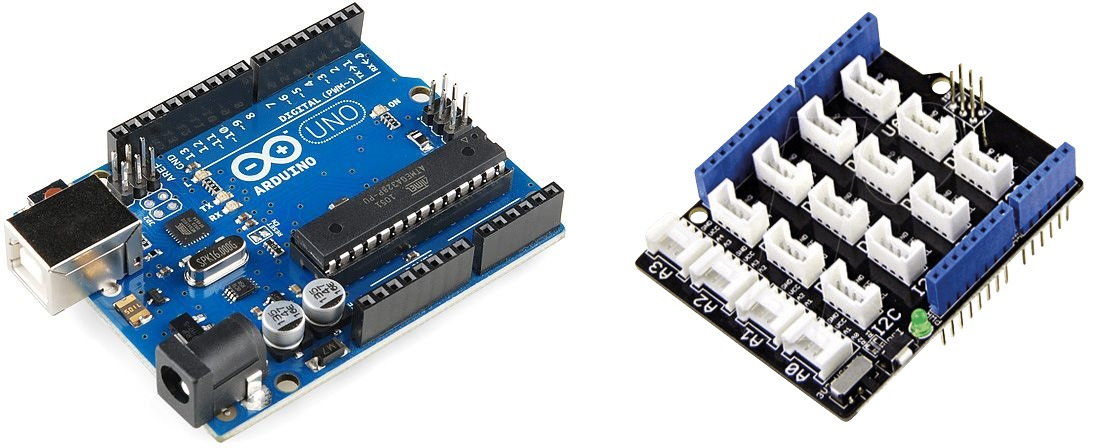
\includegraphics[width=16cm]{Bilder/arduino.jpg}
	\caption[Arduino UNO R3 (links) und Grove Base Shield]{Arduino UNO R3 (links) und Grove Base Shield\footnotemark}
\end{figure}%
\footcitetext[Bilder von:][]{Sou18, Rei18}
\newline \newline
Mit diesen Komponenten werden die vom Sensor zurückgelieferten Daten an den Arduino geleitet. Von dort aus müssen die Daten, an die mobile Applikation weitergeleitet werden. Aus diesem Grund muss an das Arduino Board ein Bluetooth-Modul angebracht werden, das Daten senden und empfangen kann. Das Empfangen von Daten ist notwendig, um die Messung zu Starten, wohingegen das Senden für die Übermittlung der Sensordaten benötigt wird. Heutige Smartphones verfügen meistens immer über eine Bluetooth-Schnittstelle, aus welchem Grund Bluetooth gut für die Übertragung geeignet ist. Eine weitere Möglichkeit wäre die Übertragung über WiFi gewesen. Das Arduino-Board wurde mit einem HC05-Bluetooth-Modul erweitert, welches Daten senden und empfangen kann. Dieses ist in Abbildung ? zu sehen.
\begin{figure}[h]
	\centering
	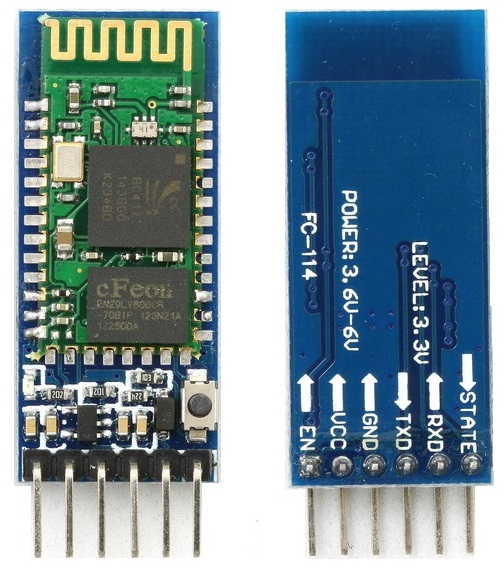
\includegraphics[width=7cm]{Bilder/hc05.jpg}
	\caption[HC-05-Bluetooth-Modul für Arduino]{HC-05-Bluetooth-Modul für Arduino\footnotemark}
\end{figure}%
\newline
Die Beschreibung der Entwicklungsarbeiten wird in zwei Teile aufgespalten. Der erste Teil ist der Quellcode des Arduinos, der zweite Teil die Entwicklung des Emotionstest in der emoTrix-App. \newline
\begin{lstlisting}[caption={Quellcode des Arduinos},style=Arduino]
#include <SoftwareSerial.h>
SoftwareSerial BTserial (10, 11); const int GSR=A0;
int sensorValue=0; int gsr_average=0;
boolean measuring = false; char BTString;

void setup(){
	BTserial.begin(9600);
}

void loop(){
	BTString = BTserial.read();
	if(BTString == 'S'){
		measuring = true;
	}
	if(BTString == 'F'){
		measuring = false;
	}
	if(measuring){
		long sum=0;
		for(int i=0;i<10;i++){ 
			sensorValue=analogRead(GSR);
			sum += sensorValue; delay(5);
		}
		gsr_average = sum/10;
		BTserial.print(gsr_average); BTserial.println( ";");
	}
}
\end{lstlisting}
In Listing ? ist der Quellcode des Arduinos abgebildet. In Zeile 1 wird die SofwareSerial-Bibliothek eingebunden, die eine Verwendung der Pins des Arduinos für verschiedene Module ermöglicht. In Zeile 2 wird dem Arduino mitgeteilt, dass auf den Pins 10 und 11 ein Bluetooth-Modul angeschlossen ist und eine Konstante (GSR) festgelegt, die auf den Anschluss A0 des Grove Shields verweist, an dem der GSR Sensor angeschlossen ist. \newline
Generell besteht der Programmcode des Arduinos immer aus zwei Bestandteilen: einem Setup-Block und einem Loop-Block. Der Setup-Block wird einmalig beim Einschalten des Arduinos ausgeführt. Danach wird der Loop-Block solange wiederholt, bis der Arduino ausgeschalten wird. 
In Zeile 7 innerhalb des Setup-Blocks wird die Geschwindigkeit der seriellen Datenübertragung der Ports des Arduinos, die mit dem Bluetooth-Modul verbunden sind. Hierbei wird die Geschwindigkeit auf 9600 Bits pro Sekunde gesetzt.\footcite[Vgl.][]{Ard18b} Dies entspricht der üblich verwendeten Geschwindigkeit und hat in Tests sehr gut funktioniert. \newline
Der Loop-Block beginnt in Zeile 11 mit dem Auslesen der Daten, die über das Bluetooth-Modul empfangen werden. Die Variable \textit{BTString} wird mit diesen Daten beschrieben. Die App muss zum Starten der App den String \textit{S} (für Start) per Bluetooth übertragen. Ist dies der Fall, wird die Variable \textit{measuring} auf true gesetzt. Mit dem String \textit{F} (für Finished) kann die App dem Arduino das Stopsignal für die Messung geben. Demenstprechend wird \textit{measuring} auf false gesetzt. Dies ist in den Zeilen 15 bis 17 umgesetzt. \newline
In Zeile 18 wird über die \textit{measuring}-Variable überprüft, ob gemessen werden soll. Wenn ja, wird eine Variable für die Summe von 10 Messdaten initialisiert. Anschließend werden in Abstand von 5 Millisekunden 10 Messungen durchgeführt. In Zeile 21 wird die eigentliche Messung des Sensors durchgeführt. Der hier verwendete GSR-Sensor liefert als Output einen Integer-Wert, der die Stromspannung auf dem seriellen Port des Arduinos in Volt entspricht. Dieser Wert hängt von der gemessenen Hautleitfähigkeit ab. Die Umrechnung in den Hautleitfähigkeit geschieht dann in der App und wird im Anschluss noch betrieben. Im Arduino-Code selbst werden die Daten überliefert, die auch der Sensor übermittelt. Alle 10 Messungen werden nach und nach aufaddiert. Dies geschieht in der for-Schleife in den Zeilen 20 bis 23. Anschließend wird die Summe durch 10 geteilt, sodass man den Durchschnitt aller 10 Werte erhält. Dieses Verfahren wird durchgeführt, da die Messdaten des Sensors Schwankungen aufweisen, die dadurch eliminiert werden können. In Zeile 25 wird schließlich der Messwert auf den Port des Bluetooth-Moduls geschickt und damit versendet. Als Trennzeichen zum nächsten Wert wird ein Semikolon angehängt. \newline
Wenn die Messung gestartet wurde, erhält die mobile Applikation also alle 50 Millisekunden vom Arduino per Bluetooth einen Integer-Wert übermittelt. \newline
Die Daten, die der Arduino schickt, müssen innerhalb der App verarbeitet werden. Hierfür wurde eine neue TestPage mit dem Namen GSRPage erstellt. Diese Page dient dazu, sich mit dem Arduino Bluetooth-Modul zu verbinden und die Messung zu starten und zu stoppen. Zusätzlich werden die gemessenen Werte in einem Graphen dargestellt, um zu veranschaulichen, wie sich die Hautleitfähigkeit während der Messung ändert. \newline \newline
Die GSRPage implementiert den GSRSensor, der eine Implementierung des Sensor-Interfaces darstellt. In der Klasse GSRSensor sind alle Methoden implentiert, die für die Umsetzug der genannten Funktionalitäten benötigt werden. In Listing 9 ist ein Ausschnitt aus der Typescript-Datei mit den wichtigsten Funktionen abgebildet. \newline \newline \newline
\begin{lstlisting}[caption={startMeasuring- und stopMeasuring-Funktion}, language=JavaScript]
startMeasuring(){
	this.bluetoothSerial.write('S').then((data: any) => { })
		.catch((e) => {
			console.log(e);
		});;
}

stopMeasuring(){
	this.bluetoothSerial.write('F').then((data: any) => {})
		.catch((e) => {
			console.log(e);
		});
}
\end{lstlisting}
Die Funktion \textit{startMeasuring} implementiert das Starten der Messung. Für die GSRPage wurde das Ionic-Package Bluetooth Serial hinzugefügt, das Bluetooth-Optionen des Smartphones für die App verfügbar macht. Das Package wird hier mit \textit{this.bluetoothSerial} referenziert. Das Pairen und Verbinden des Smartphones mit dem Bluetooth-Modul ist selbsterklärend (über eine \textit{connect}-Methode) und deswegen im Listing nicht aufgeführt. Nachdem die Verbindung eingerichtet wurde, kann die \textit{startMeasuring}-Funktion aufgerufen werden. Dabei wird in Zeile 2 mit \textit{write} ein String an das verbundene Bluetooth-Modul gesendet. Wie bereits beschrieben muss zum Start der String \textit{S} gesendet werden. Falls ein Fehler auftritt, wird dieser in Zeile 4 geloggt. Wenn alles ordnungsgemäß funktioniert, empfängt der Arduino den String und startet anschließend die Messung.\newline
Die \textit{stopMeasuring}-Funktion funktioniert analog zur \textit{startMeasuring}-Funktion mit dem Unterschied, dass hier der String \textit{F} zum Stoppen der Messung gesendet wird.
\newline
In Listing 6 ist implementiert, dass das Bluetooth des Smartphones auf einen neu eintreffenden Integer-Wert des Arduinos reagieren kann. Das BluetoothSerial dient dabei als Observable, den die App abonnieren kann. Dies bedeutet, dass die App darauf hingewiesen wird, wenn neue Daten angekommen sind. Mit \textit{subscribe(";")} wird die App jedes Mal informiert, wenn ein Semikolon übertragen wurde. Das Semikolon wurde im Arduino-Code als Trennzeichen eingesetzt und signalisiert, dass ein Integer-Wert abgeschlossen ist. Mit dem nächsten \textit{subscribe} wird bestimmt, was ausgeführt wird, wenn ein Semikolon empfangen wird. Als \textit{data} (Zeile 1, Ende) wird immer alles übertragen, was seit dem letzten Ausführen der Funktion übertragen wurde. Es handelt sich also immer um einen Integer-Wert und das Semikolon. In Zeile 2 wird aus diesem Grund das letzte Zeichen der Übertragung abgeschnitten, sodass der \textit{value}-Variable nur der Integer-Wert zugewiesen wird.
In Zeile 3 folgt die Umwandlung des Integer-Wert, der der Stromspannung auf dem seriellen Port entspricht, in den Hautwiderstand. \newline
\begin{lstlisting}[caption={Verarbeitung der Sensordaten}, language=JavaScript]
this.bluetoothSerial.subscribe(";").subscribe(function (data){
		self.value = data.substring(0,data.length - 1);
		self.value = ((1024+2*self.value)*10000)/(512-self.value);
		if(self.time%5 == 0){
			if(self.time != 0){
				var data: any = {value: self.value, oldValue: self.oldValue};
				self.GsrSensor.onSensorData(data);
			}
			self.oldValue = self.value;
		} 
		if(self.time%20 == 0){
			self.sensorObserver.next("Update Graph");
		}
		self.time++;
	}, function (error){
		console.log(error);
});
\end{lstlisting}
Nach Herstellerangaben kann mit der Formel \textit{(1024+2*x)*10000)/(512-x)} der Hautwiderstand berechnet werden, wobei x der gemessenen Stromspannung entspricht.\footcite[Vgl.][]{Gro18} Warum diese Formel genau so aussieht, hat mit dem internen Aufbau des Sensors zu tun, der aus Analog-Digital-Umsetzern und Verstärker aufgebaut ist. \footcite[Vgl.][1. Forumsantwort]{Com18} Da die genaue Erklärung der Formel sehr komplex ist und den Rahmen der Arbeit sprengen würde, wird die Formel hier nicht weiter thematisiert. Wichtig ist, dass man durch diese Umrechnung man den Hautwiderstand des Benutzers in Ohm erhält. \newline
Da alle 50 Millisekunden ein Wert übertragen wird, wird kein neuer Timer benötigt. Dieser wurde anfangs mit dem Wert 0 initialisiert und in Zeile 14 nach jedem neuen Wert um 1 erhöht. Da ein Wert und damit eine Verabeitung alle 50ms für die App einen sehr hohen Workload bedeutet würde, wird nur jeder fünfte übertragene Wert betrachtet. Dies ist in Zeil 4 mit einer if-Bedingung umgesetzt. In Zeile 6 werden immer zwei aufeinander folgende Ohm-Werte zusammengefasst und anschließend in Zeile 7 die onSensorData-Methode mit diesen Daten aufgerufen. Zwei Werte sind für den Mapper trivialerweise genug, um zu schauen ob der Wert gestiegen oder gesunken ist. Da am Anfang nur der erste Wert vorhanden ist, wird dieser Fall in Zeile 5 abgefangen. Das Setzen des alten Werts (\textit{oldValue}) geschieht in Zeile 9. \newline
In Zeile 11 bis 13 wird implementiert, das außerdem jeder zwanzigste Wert in einem Graphen auf der GUI eingetragen wird. Dazu wird die Observer-Funktion des Sensors genutzt und die Information, dass der Graph geupdatet werden muss, an die GSRPage weitergeleitet, die mit \textit{subscribe()} den Sensor abonniert hat. Eine häufigere Darstellung als jeder zwanzigste Wert ist ebenfalls nicht sehr vorteilhaft für die Benutzung der App, da dies sehr rechenlastig ist. Der Trend des Graphen ändert sich außerdem nicht wesentlich, wenn nicht jeder einzelne übertragene Datenpunkt eingetragen wird. In Zeile 15 bis 17 wird letzlich noch das Error-Handling implementiert. \newline
Abschließend muss nun noch die Implementierung des Mappers der GSRSensor-Klasse vorgestellt werden. Dieser ist in Listing ? abgebildet. \newline
\begin{lstlisting}[caption={Mapper des GSR-Sensors}, language=JavaScript]
mapper(data: any): IndicatorScore[]{
	let newIndicatorScore: IndicatorScore;
	if(data.value > data.oldValue){
		newIndicatorScore = {indicator: "activation", score: 0};
	} else if (data.value < data.oldValue){
		newIndicatorScore = {indicator: "activation", score: 1};
	} else { 
		newIndicatorScore = {indicator: "activation", score: 0.5};
	}
	return [newIndicatorScore];
}
\end{lstlisting}
Die Funktionsweise des Mappers ist nicht sonderlich komplex. Wie bereits beschrieben, erhält der Mapper per onSensorData-Funktion zwei Werte: den aktuellen Sensorwert (\textit{value}) und den vorherigen Sensorwert (\textit{oldValue}). Je nachdem, wie der Wert sich verändert hat, wird die in Zeile 2 initialisierte Variable \textit{newIndicatorScore} unterschiedlich initialisiert. Wenn der Wert gestiegen ist, dann ist auch der Hautwiderstand gestiegen. Somit ist dies ein Zeichen für Entspannung und kein Anzeichen für Aktivation. Aus diesem Grund wird, wenn die Prüfung in Zeile 3 zutrifft, in Zeile 4 die Variable mit einem IndicatorScore initialisiert, der den Indicator \textit{activation} auf 0 setzt. Ist der Wert gesunken (siehe Prüfung in Zeile 5), so ist auch der Hautwiderstand gesunken, aus welchen Grund hier in Zeile 6 der \textit{activation}-Indicator mit 1 initialisiert wird.  Falls keine der Prüfungen in Zeile 3 und 5 zu, dann ist der Wert gleich geblieben und es gibt kein Anzeichen für oder gegen Aktivation. Aus diesem Grund hat die \textit{activation} in diesem Fall den Score 0.5 (Zeile 8). Der GSR-Sensor beeinflusst nur den \textit{activation}-Indikator und deswegen kann die Variable \textit{newIndicatorScore} alleine in einem Array in Zeile 10 zurückgegeben werden. 
\subsubsection{Face-Test}
\subsubsectionauthor{Torben Brenner}
Eine der am höchsten priorisierten Erfassungsmöglichkeiten für Emotionen, war die Messung der Emotionen anhand der Mimik des Menschen mithilfe der Smartphonekamera. Wie im Mockup\footnote{siehe \ref{section:Mockup-Gesichtserkennung} S.\pageref{section:Mockup-Gesichtserkennung}} beschrieben soll der Nutzer zuerst ein Bild machen können und sich dieses anzeigen lassen können, bevor es ausgewertet werden soll. Wenn das Bild zur Analyse freigeben wird, soll dem Nutzer ein Ladebildschirm angezeigt werden. Die Analyse selbst wird nicht auf dem Smartphone durchgeführt, sondern mit Hilfe der Gesichtserkennungsschnittstelle von Microsoft\footcite[siehe ][]{Mic18}.\newline
Zu Beginn der Entwicklung wurde eine Komponente entwickelt, welche das Schießen eines Fotos ermöglicht. Ionic-Komponenten bestehen aus einem HTML-Template, einer SCSS Datei und einem TypeScript Script. Diese Aufteilung in drei Dateien ermöglicht eine Trennung von grafischer Darstellung und der Logik. Die grafische Darstellung der Komponente besteht aus einem Bild, dass nur angezeigt wird wenn mit der Komponente auch ein Bild gemacht wurde, und einem \textit{Ionic-Button}, der das Fotografieren auslöst. Interessanter ist die Logik der Komponente, die daraus besteht abhängig von der der Auswahl des Entwicklers entweder ein Bild zu machen oder eine Videoaufnahme zu starten. Dies wird mit der Übergabe eines Input Parameters ermöglicht. \newline
\begin{lstlisting}[caption={Input und Output der Kamera Komponente}, language=JavaScript]
	@Input() pictureMode: boolean;
	@Output() sourceChanged: EventEmitter<String> = new EventEmitter<String>();
\end{lstlisting}
Da die Komponente aber auch die Bilder, die mit ihr gemacht wurden, herausgeben soll wird ein \textit{Output} definiert. Dieser wird mit Hilfe eines EventEmitters realisiert, der ein Event auslöst auf das andere Teile der Anwendung, die eine Kamera Komponente implementieren reagieren können. Das Event gibt hierbei einen String aus, der in diesem Test dem Base64 codierten Bild entspricht. Im folgenden zusehen ist die Einbindung der Kamera Komponente in den Face-Test. \newline \newline
\begin{lstlisting}[caption={Einbindung Kamera Komponente}, language=HTML]
	<camera [pictureMode]="true" (sourceChanged)="onSourceChanged($event)"></camera>
\end{lstlisting}
Das Fotografieren wird in Ionic mit Hilfe einer \textit{native} Komponente umgesetzt. Diese Komponente erlaubt den plattformunabhängigen Zugriff auf die Kamera\footcite{Ion18e}. Dazu wird in der App direkt eine Weiterleitung an die ausgewählte Kamera App des Nutzers durchgeführt. Nachdem der Nutzer mit dieser ein Bild gemacht hat, kann entweder der Speicherort oder das Bild selbst zurückgegeben werden. Der zurückgegebene Wert wird dann von der Kamera Komponente per \textit{EventEmitter} ausgegeben.\newline
Wie in der Einbindung der Komponente zu sehen ist, wird beim auslösen des Events \textit{sourceChanged} im Face-Test eine Funktion aufgerufen. Dies geschieht mittels \textit{Event Binding}. Die aufgerufene Funktion speichert den empfangenen Source Wert in einer lokalen Variable im Face-Test. Bei Betätigung des \textit{Send Picture Buttons} wird daraufhin die Analyse gestartet. Die Analyse wird von der \textit{FaceSensor} Klasse durchgeführt. Dazu wird vom Face-Test die Funktion \textit{prepareData} aufgerufen, die eine HTTP POST Anfrage an die Microsoft Gesichtserkennungsschnittstelle durchführt. Die Details der Anfrage sind in folgender Codeausschnitt zu sehen: \newline
\begin{lstlisting}[caption={Aufbau Anfrage an Gesichtserkennungsschnittstelle}, language=JavaScript]
{
	url: 'https://westeurope.api.cognitive.microsoft.com/face/v1.0/detect?returnFaceAttributes=emotion',
	type: 'POST',
	processData: false,
	headers: {
		'Ocp-Apim-Subscription-Key': '{Api Key}'
	},
	contentType: 'application/octet-stream',
	data: this.makeblob(base64Data)
}
\end{lstlisting}
Das einzig nennenswerte an dieser Anfrage ist die Übertragung des Base64 codierten Bildes. Diese geschieht nämlich in Form eines Blob(Binary Large Object). Laut \textit{MDN web docs} ist ein Blob eine ``dateiähnliche Menge unveränderlicher Roh-Daten''\footcite[Vgl. ][Abschnitt Übersicht]{Mdn18}. Diese wird nicht nur bei der Übertragung großer Datenmengen verwendet, sondern auch beim Abspeichern größerer Dateien in Datenbanken. Um das Base64 codierte Bild in einen Blob zu übertragen wurde die Hilfsmethode \textit{makeblob} genutzt. Diese wurde nicht von mir selbst entwickelt sondern von Kalpesh Singh\footcite[Vgl. ][Antwort von Kalpesh Singh]{Sin16}. Die Funktion trennt die \textit{ContentType} Informationen von den Roh-Daten und überträgt diese dann in einen neuen Blob. Bei der Base64 Codierung müssen die Roh-Daten erst mit Hilfe der JavaScript Funktion \textit{charCodeAt} in Ganzzahl Werte übertragen werden. Der generierte Blob wird dann im \textit{Body} der HTTP Anfrage mit übertragen.\newline
Nach dem senden der Request wird auf der Oberfläche der App dem Nutzer mit Hilfe eines \textit{Ionic Loaders}\footcite{Ion18f} signalisiert, dass im Hintergrund gerade eine Verarbeitung der Daten stattfindet. Da die Sensor Klasse ein sogenanntes \textit{Observable} implementiert, können Statusmeldungen zwischen der Face-Test Seite und dem \textit{FaceSensor} ausgetauscht werden. Die Statusmeldungen werden auf Seiten des \textit{FaceSensor} initiert und von der Seite mit Hilfe einer \textit{Callback} Funktion verarbeitet. \newline
\begin{lstlisting}[caption={Callback Methode auf FaceSensor Observable}, language=JavaScript]
	this.faceSensor.observable.subscribe(data => {
		if(data == "Sending data to Microsoft"){
			this.loader.present();
		}
		if(data == "empty result"){
			this.loader.dismiss();
			alert("Microsoft Server couldn't recognize your face. Please make sure your face is visible");
		}
		if(data.startsWith("result:")){
			console.log("This is a result");
			this.loader.dismiss();
			let emotions = JSON.parse(data.replace("result:", ""));
			console.log(emotions);
			this.faceSensor.onSensorData(emotions);
		}
		if(data.startsWith("error:")){
			this.loader.dismiss();
			let errorString = data.replace("error:", "");
			alert(errorString);
		}
	});
\end{lstlisting}
Die Daten des \textit{FaceSensor} werden mit Strings übertragen. Durch das Schlüsselwort ``result'' wird gekennzeichnet, das es sich beim Rest des Strings um Ergebnis Daten handelt, die mit der \textit{JSON.parse} Methode in ein JavaScript Objekt übertragen werden können. Durch ``error'' wird gekennzeichnet, dass ein Fehler aufgetreten ist der ausgegeben werden soll. Dies wird mit Hilfe eines \textit{alert} umgesetzt. Es kann außerdem passieren, dass die Microsoft Gesichtserkennungsschnittstelle kein Gesicht erkennt. Das ist in unseren Testläufen insbesondere dann aufgetreten, wenn das Bild um 90 Grad gedreht war. Für diesen Fall haben wir eine eigene Fehlernachricht eingebaut.\newline
Wenn aber alles ohne Fehler abgelaufen ist, erhalten wir vom Microsoft Server ein JSON Objekt der Form: \newpage
\begin{lstlisting}[caption={Ergebnis Gesichtserkennungsschnittstelle, Beispiel Microsoft}, language=JavaScript]
[
	{
		"faceId": "579838a9-fb50-4333-8770-32858b2d0fc6",
		"faceRectangle": {
			"top": 131,
			"left": 177,
			"width": 162,
			"height": 162
		},
		"faceAttributes": {
			"emotion": {
				"anger": 0,
				"contempt": 0,
				"disgust": 0,
				"fear": 0,
				"happiness": 0.001,
				"neutral": 0.987,
				"sadness": 0.001,
				"surprise": 0.01
			}
		}
	}
]
\end{lstlisting}
Aus diesem Objekt interessiert uns der Datensatz \textit{emotion}. Diesen kann man mittels JavaScript einfach auslesen. Eine Problematik die derzeit nicht im Face-Test behandelt wird, ist die Verarbeitung von mehreren Gesichtern in einem Bild. In diesem Fall würde ein weiteres Objekt mit einer anderen \textit{faceId} zurückgegeben werden. Für die Zukunft wäre es denkbar die \textit{faceId} in der Ausgabe zu kontrollieren und den Nutzer zur Identifikation ein erstes Bild machen zu lassen in dem die \textit{faceId} ermittelt wird. Dies wäre zum Beispiel in den Settings möglich. Problematisch an diesem Ansatz ist aber, dass die \textit{faceId} nur temporär ist und nach 24 Stunden abläuft. Also müsste der Nutzer nach einem Tag Inaktivität diese neu setzen.\newline
Zum Abschluss des Face-Tests fehlt nur noch die Implementierung der \textit{mapper} Funktion im \textit{FaceSensor}. Diese ist relativ einfach, da der Funktion einfach das \textit{emotion} Objekt aus der HTTP Antwort weitergegeben werden kann. Dort werden die Werte dann in \textit{IndicatorScores} übertragen, was in diesem Fall trivial ist, da Sie bereits Prozente darstellen und somit einfach übernommen werden können. Das senden der Daten an den Decider wird durch die Funktion \textit{onSensorData} der Klasse \textit{Sensor}, von der der \textit{FaceSensor} erbt, bereits übernommen, womit die Implementation abgeschlossen ist.   
\subsection{Beschreibung der implementierten Kausalitätsregeln}
\subsectionauthorlong{Torben Brenner}
Alle von uns implementierten Kausalitätsregeln befinden sich aus Übersichtsgründen in der Datei \textit{CausalityRulesArray.ts}. Hier werden zum aktuellen Zeitpunkt sechs verschiedene Kausalitätsregeln implementiert(zwei davon für den GSR-Test und vier für den Face-Test). Diese Regeln werden zusammen in einem Array exportiert, welches von der \textit{Decider} Klasse eingebunden wird. Im folgenden sollen die verschiedenen Regeln genauer erläutert werden.
\subsubsection{Regeln des GSR-Test}
\subsubsectionauthor{Torben Brenner \& Lukas Seemann}
Da der \textit{Activation} Indikator entweder \textit{0, 0.5 oder 1} sein kann, ist es nur notwendig zwei Regeln für diesen zu implementieren. Wenn der \textit{Activation} Indikator einen Wert von 0.5 hat, ist dieser als neutral anzusehen, d.h. die vom GSR-Sensor erfassten Werte zeigen keine Tendenz für den Stress. In diesem Fall finden keine Veränderungen an den \textit{EmotionScores} statt, weshalb hierfür auch keine Kausalitätsregel zu implementieren ist. Anders sieht das bei den Werten \textit{0 und 1} aus. In diesen Fällen zeigt sich eine Tendenz der erfassten Werte für emotional erregt (1) oder nicht emotional erregt (0). Deshalb unterscheidet sich die Bedingung der beiden Regeln gerade mal durch die Prüfung auf den bestimmten \textit{score}. \newline
\begin{lstlisting}[caption={Bedingung der ersten Kausalitätsregel (emotional erregt)}, language=JavaScript]
	(indicatorScore: IndicatorScore) => {
		return indicatorScore.indicator == <indicator>"activation" && indicatorScore.score == 1;
	}
\end{lstlisting}
Auch die Auswirkungen der beiden Regeln sind sich ähnlich. So werden bei Eintritt der ersten Regel zu den \textit{EmotionScores} für die Emotionen \textit{wütend, fröhlich und überrascht} jeweils eins zu dem Score hinzu addiert. Bei Eintritt der zweiten Regel wird stattdessen eins subtrahiert. Diese Änderungen wirken zwar sehr klein im Vergleich zu den Änderungen der Kausalitätsregeln des Face-Test, werden sich aber aufgrund der Menge von Daten in einem Zeitraum dennoch bemerkbar machen. So werden in einer Sekunde circa 20 Werte erfasst, während dem der Face-Test deutlich länger für die Durchführung benötigt.
\subsubsection{Regeln des Face-Test}
\subsubsectionauthor{Torben Brenner}
Für den Face-Test wurden vier Kausalitätsregeln definiert. Von diesen vier Regeln ist jeweils eine für einen bestimmten \textit{EmotionScore}. Da bei der Eignung des Gesichts als Emotionsindiz festgestellt wurde, dass dieses äußert aussagekräftig ist werden die durch den Face-Test erfassten Werte sehr stark gewichtet. Die Werte die vom Test ermittelt werden sind Prozentzahlen, die aussagen wie wahrscheinlich eine bestimmte Emotion ist. Deshalb wird bei der Erfassung eines solchen Wertes dieser mit 100 multipliziert und dann auf den jeweiligen \textit{EmotionScore} addiert. \newline
\begin{lstlisting}[caption={Kausalitätsregel basierend auf Face-Test für Emotion Wut}, language=JavaScript]
	(indicatorScore: IndicatorScore) => {
		return indicatorScore.indicator == <indicator>"angryIndicator" && indicatorScore.score != undefined;    
	},[
		(data: EmotionScore[], indicatorScores :IndicatorScore[]) => {
			let angry = data.find((emotionScore) => {return emotionScore.emotion == <emotion>"angry"});
			let angryIndicator = indicatorScores.find((indicatorScore) => {return indicatorScore.indicator == <indicator>"angryIndicator"});
			angry.score = angry.score + (100 * angryIndicator.score);
			return data;
		}
	]
\end{lstlisting}
Als Bedingung das eine Kausalitätsregel des Face-Test eintritt, ist gewählt das der jeweilige Indikator definiert ist. Diese sind im Normalfall nicht definiert, werden aber bei Erfassung eines Bildes gesetzt. Im Falle der Wut ist der Indikator der sogenannte \textit{angryIndicator}. Bei Eintritt der Bedingung werden die Auswirkungen wie oben beschrieben ausgeführt. Die andern drei Regeln für den Face-Test unterscheiden sich nur durch die Auswahl des \textit{Indicator-} und \textit{EmotionScores}. \newline 
\subsection{Benutzeroberfläche der App}
\subsectionauthor{Lukas Seemann}
In diesem Kapitel wird die Benutzeroberfläche der mobilen Applikation beschrieben. Das Kapitel soll auch als Benutzungsanleitung für die einzelnen Funktionen der App dienen.
\subsubsection{HomePage}
\subsubsectionauthor{Lukas Seemann}
In Abbildung ? ist der StartScreen der App zu sehen. Dieser wird aufgerufen, wenn der User die App öffnet. Hier werden dem User alle Emotionstests aufgelistet, die er durchführen kann. Durch ein Klicken auf das Label oder den Pfeil gelangt der User auf den Screen des jeweiligen Tests. Von den aufgelisteten Tests wurde der Keyboard Scanner nicht umgesetzt. Ein Klicken auf dieses Label führt zu einer Meldung, dass die Seite noch nicht implementiert wurde. \newline
Führt der User einen Emotionstest erfolgreich durch, verwandelt sich bei der Rückkehr auf die HomePage der Pfeil am Ende des Test in einen Haken. So erhält der User einen Überblick darüber, welche Test er bereits durchgeführt und welche noch offen sind. \newline
Durch ein Klicken auf den \textit{Auswertung}-Button wird eine Auswertung der Testergebnisse durchgeführt, die zum Zeitpunkt des Klickens im Decider hinterlegt sind. Der User wird anschließend zur DecisionPage navigiert, welche ihm seine Ergebnisse visualisiert. \newline
\begin{figure}[h]
	\centering
	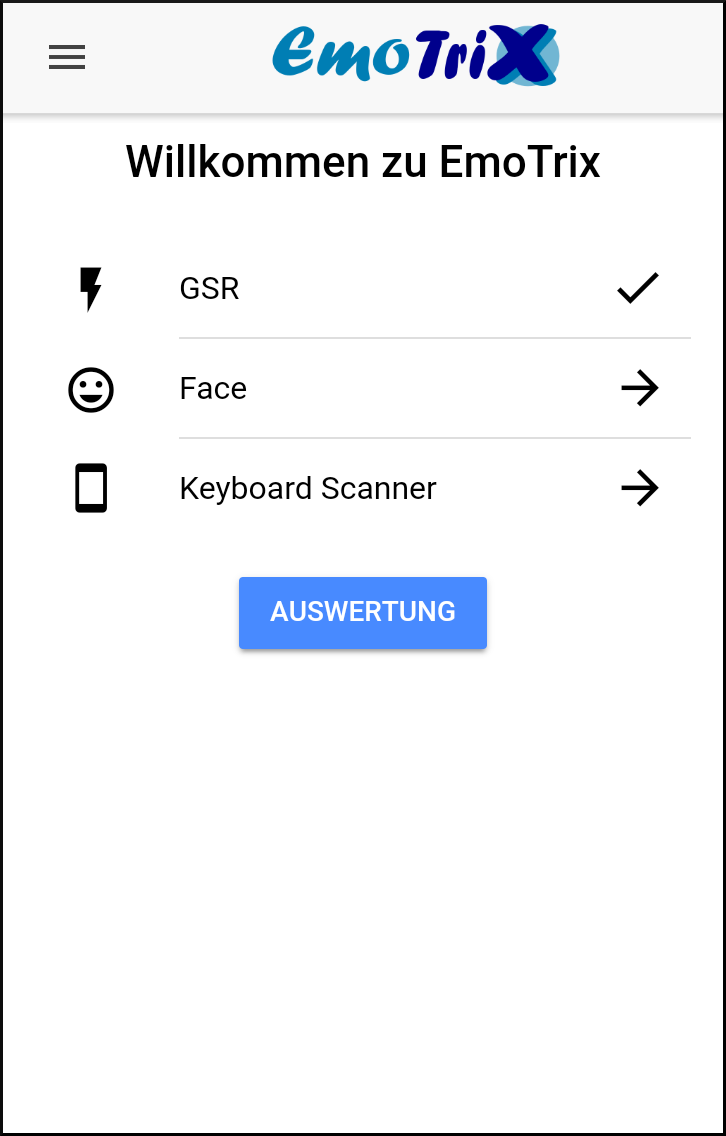
\includegraphics[width=6cm]{Bilder/homepage.png}
	\caption[GUI der HomePage]{GUI der HomePage}
\end{figure}%
\newline
Über das Klicken der drei Striche in der Toolbar oder ein Swipen nach rechts, wird seitlich ein Menü angezeigt, über welches der User zu weiteren Screens der App gelangen kann. Wie bereits im Mockup beschrieben, gibt es hier die Möglichkeiten auf eine Anleitungsseite, eine Übersicht der durchgeführten Messungen oder eine Einstellungsseite zu gelangen. Aus Zeitgründen konnte hiervon nur die Anleitungsseite umgesetzt werden. Über dieses seitliche Menü kann der User außerdem auch auf jeder beliebigen Seite über die erste Auswahlmöglichkeit (\textit{Home}) zurück zum Startscreen gelangen.
\subsubsection{GSRPage}
\subsubsectionauthor{Lukas Seemann}
Die GSRPage ist im Wesentlichen genau so umgesetzt worden, wie das Mockup den Screen vorgesehen hat. In Abbildung ? sind zwei Beispiele gezeigt, was der User auf der GSRPage sehen kann. \newline
\begin{figure}[h]
	\centering
	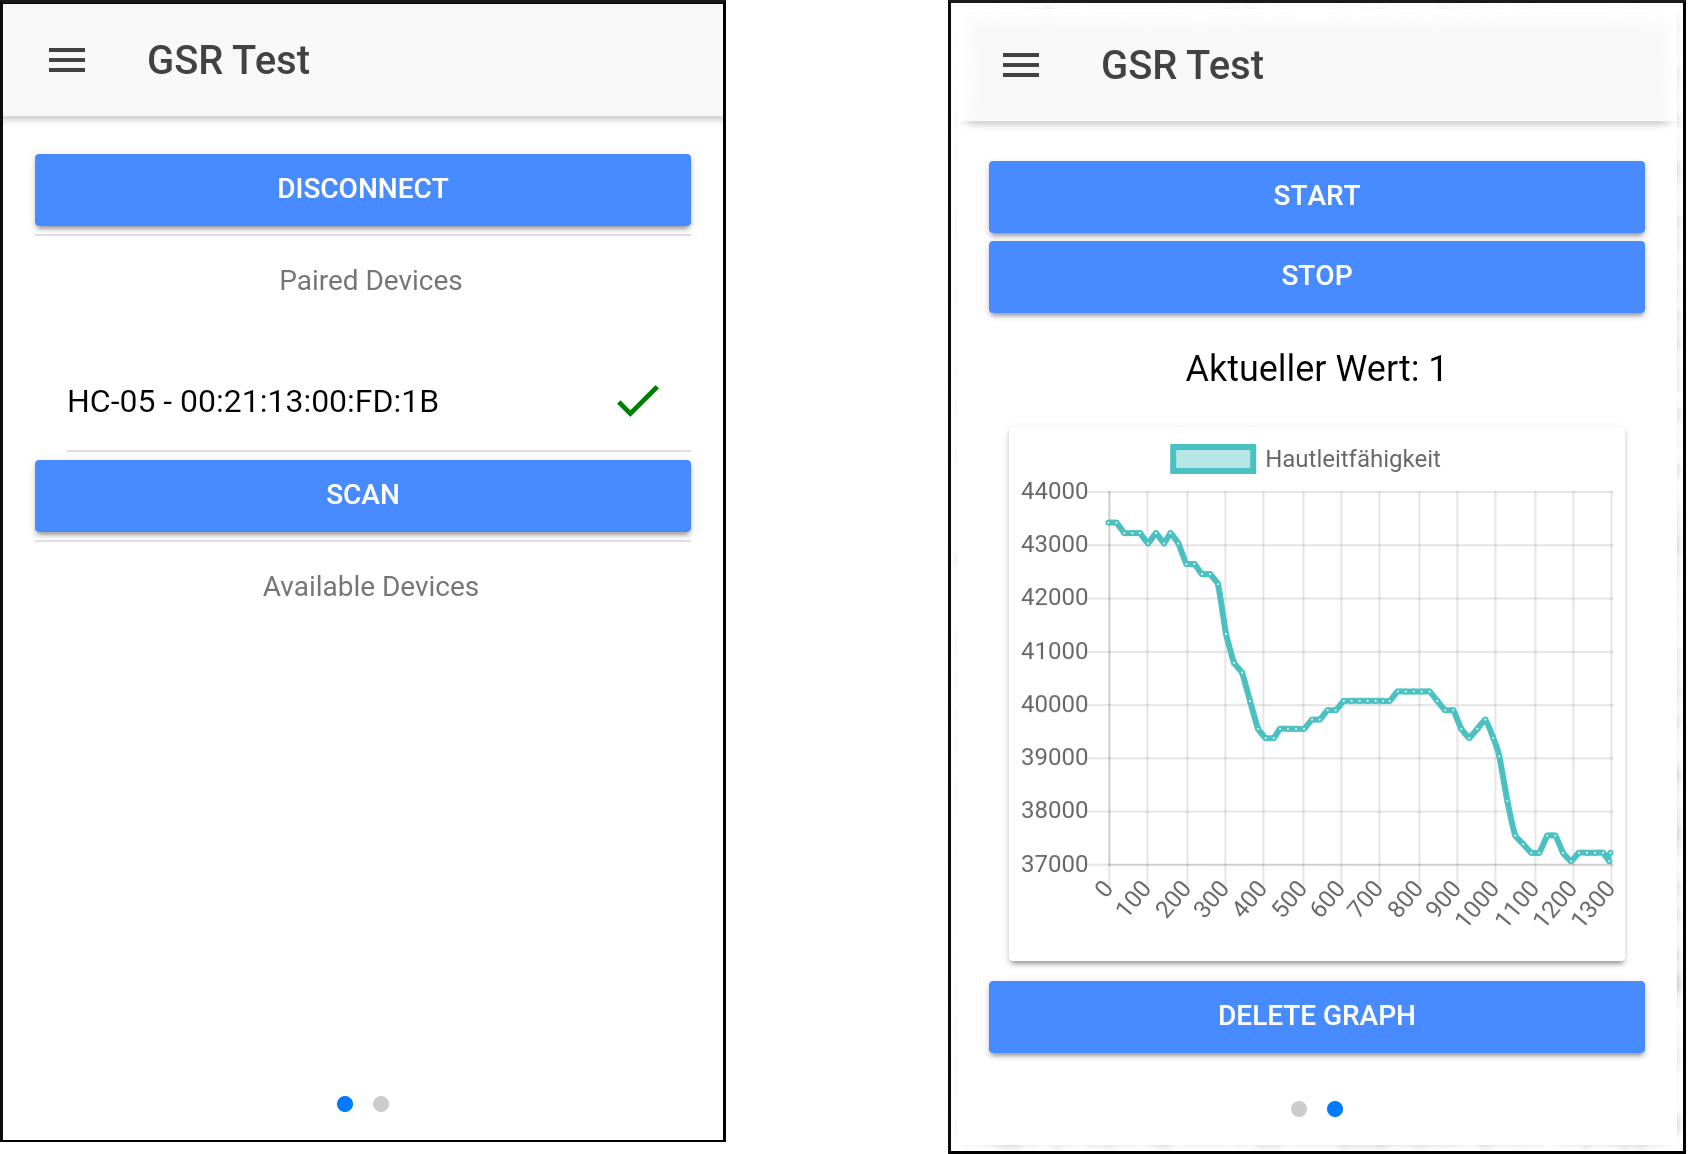
\includegraphics[width=13.5cm]{Bilder/gsrpage.png}
	\caption[GUI der GSRPage]{GUI der GSRPage}
\end{figure}%
\newline
Die GSRPage besteht aus 2 Slides, zwischen denen per Swipen hin und  her navigiert werden kann. Der erste Slide befasst sich mit dem Verbinden mit dem Bluetooth-Modul des Arduinos. Wie bereits im Mockup beschrieben, kann der User mit dem Button \textit{Scan} nach nicht verbundenen HC-05-Modulen suchen. Alle Ergebnisse werden dann unter \textit{Available Devices} angezeigt. \newline Unter \textit{Paired Devices} werden alle Bluetooth-Module gezeigt mit denen der User sich bereits schon vorher verbunden hat. Durch Klicken auf einen Eintrag in \textit{Paired Devices} oder nach dem \textit{Scan} in \textit{Available Devices} erscheint eine Anzeige, ob der User sich gerne mit dem Modul verbinden möchte. Bestätigt er dies und die Verbindung ist erfolgreich, wird dies durch einen grünen Haken nebem dem Eintrag angezeigt. Damit ist das Verbinden mit dem Bluetooth-Modul abgeschlossen und der Test kann gestartet werden. \newline
Durch ein Swipen nach rechts gelangt man auf den Screen, um den Test zu starten. Der Benutzer muss nun die Elektroden des GSR-Sensors an die mittleren Fingerkuppen des Zeige- und Mittelfinger der schwachen Hand anbringen. Durch Drücken des \textit{START}-Buttons wird die Messung gestartet. Danach wird der Hautwiderstand des Benutzers in Echtzeit in den Graphen eingetragen, der in der Mitte des Screens zu sehen ist. Wenn der Graph sinkt, bedeutet dies, dass die Hautwiderstand sinkt und somit der User emotional erregt wird. Eine Steigung des Graphen hingegen bedeutet einen gesteigerten Hautwiderstand und somit Entspannung. Hierbei sei nochmals angemerkt, dass der Körper ungefähr 4 Sekunden benötigt, dass die Aktivation sich anhand des Schweißausstoßes feststellen lässt. Ein schnelles Ein- und Ausatmen führt bei den meisten Menschen beispielsweise dazu, dass der Graph nach 4 Sekunden anfängt zu sinken. \newline
Während die Messung läuft kann der User beliebig weiter durch die App navigieren, da der Sensor weiterhin im Hintergrund Messwerte einsammelt. In dieser Zeit der Messung ist sogar für interessantere Ergebnisse angedacht, dass andere Emotionstest durchgeführt werden. Wenn auf die GSRPage zum Graphen zurückgekehrt wird, findet der User dieser wieder im aktuellen Stand und der Graph wird weiterhin aktualisiert. Durch Klicken auf den \textit{STOP}-Button wird die Messung beendet. Durch diesen Button wird auch der Haken für den GSR Test auf der HomePage gesetzt. Der User kann theoretisch zu jeder Zeit eine neue Messung starten und beenden. Jede Messung wird am Ende in der Auswertung berücksichtigt. \newline
Durch Klicken des \textit{DELETE GRAPH}-Buttons kann der User außerdem den Graph zurücksetzen. Dies kann aus Übersichtlichkeitsgründen sinnvoll sein, wenn der User gerne den Graphen neu starten lassen möchte. Das Drücken des Buttons ändert allerdings nicht, dass alle gemessenenen Daten an den Decider gesendet werden.
\subsubsection{CameraPage}
\subsubsectionauthor{Lukas Seemann}
Die CameraPage dient dazu, den Emotionstest der Gesichtserkennung auszuführen. Auch diese Page konnte so umgesetzt werden, wie es in den Mockups geplant wurde. Die GUI der CameraPage ist in Abbildung ? gezeigt. \newline
\begin{figure}[h]
	\centering
	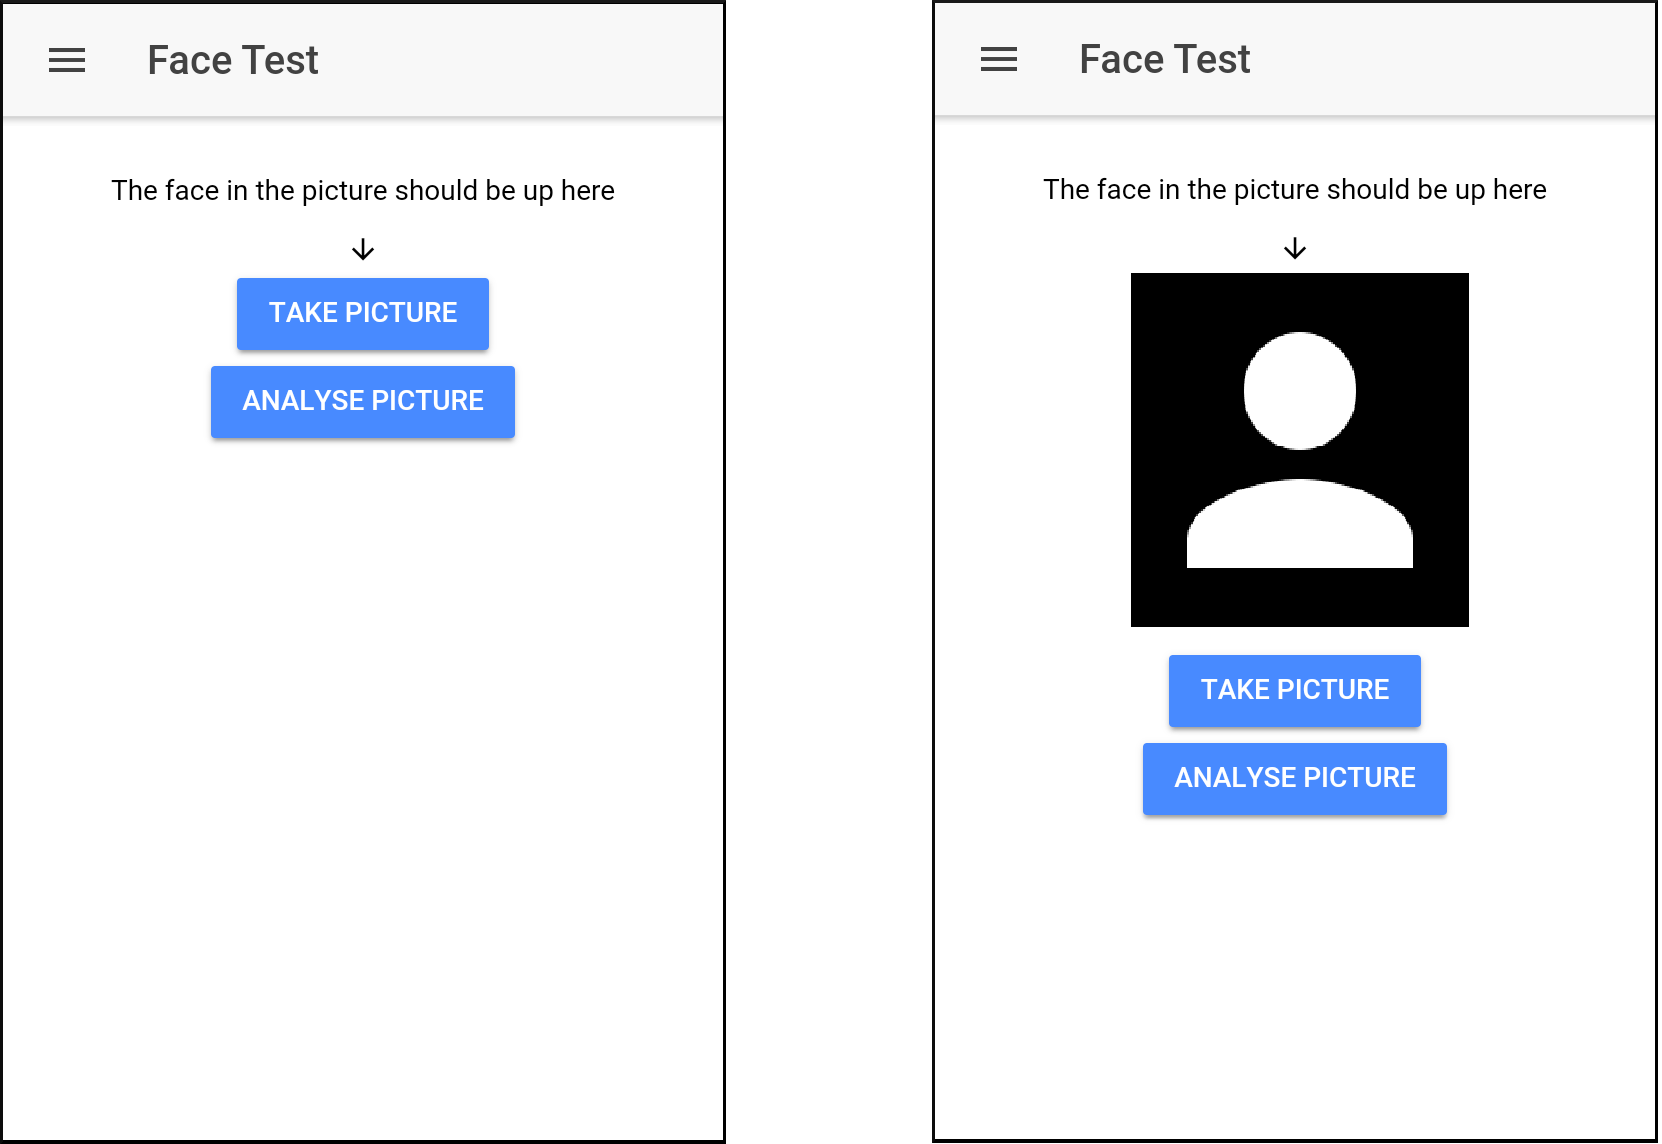
\includegraphics[width=13.5cm]{Bilder/camerapage.png}
	\caption[GUI der CameraPage]{GUI der CameraPage}
\end{figure}%
\newline
Mithilfe des \textit{TAKE PICTURE}-Buttons kann der User ein Bild von sich selbst aufnehmen. Beim ersten Benutzen der App wird beim Drücken dieses Buttons ein Hinweis angezeigt, dass der User bestätigen muss, dass die App emoTrix Zugriff auf die Kamera benötigt. Ansonsten wird die Kamera des Smartphone aufgerufen. Anschließend muss ein Bild vom Gesicht des Nutzers aufgenommen, welches im Anschluss von der API analysiert werden soll. Das aufgenommene Bild wird dann, wie rechts abgebildet, auf dem Screen der App eingefügt. Hierbei muss darauf geachtet werden, dass das Gesicht des Users auf dem Bild nach oben zeigt. Ist dies nicht der Fall muss ein neues Bild durch erneutes Drücken des \textit{TAKE PICTURE}-Buttons aufgenommen und das Smartphone entsprechend gedreht werden, dass das Bild in der richtigen Anordnung in der App angezeigt wird. Die API ist ansonsten nicht in der Lage, das Foto zu analysieren. \newline
Wird das gewünschte Foto in richtiger Anordnung auf dem Screen angezeigt, kann der User mit dem \textit{ANALYSE PICTURE}-Button das Bild an die Microsoft API senden. Anschließend erscheint ein Loading-Anzeige, die anzeigt, dass das Bild übertragen wird. Verschwindet diese Lade-Anzeige ohne Fehlermeldung, wurde das Bild übertragen und das Bild analysiert. Die Ergebnisse sind dann bereits in den Decider eingetragen worden und der Test ist abgeschlossen. Nach einem analysierten Bild wird auch der Teststatus auf der HomePage auf erledigt gesetzt. Natürlich ist es jedoch möglich und auch gewünscht, dass der User mehrere Bilder analysieren lässt. Dadurch wird die Auswertung am Ende umfangreicher und realitätsgetreuer. Außerdem ist es auch sinnvoll, während einer Hautwiderstandsmessung-Bilder analysieren zu lassen, da dies ebenfalls zu aussagekräftigeren Ergebnissen führt.
\subsubsection{DecisionPage}
\subsubsectionauthor{Lukas Seemann}
Drückt der User auf der HomePage auf den \textit{AUSWERTUNG}-Button wird er an die DecisionPage weitergeleitet. Beim Aufrufen dieses Screens werden alle IndicatorScores, die sich zu diesem Zeitpunkt im \textit{data}-Array des Deciders befinden, zu Emotionscores umgewandelt. Auch die DecisionPage konnte wie geplant umgesetzt werden und sind in Abbildung ? abgebildet. \newline 
\begin{figure}[h]
	\centering
	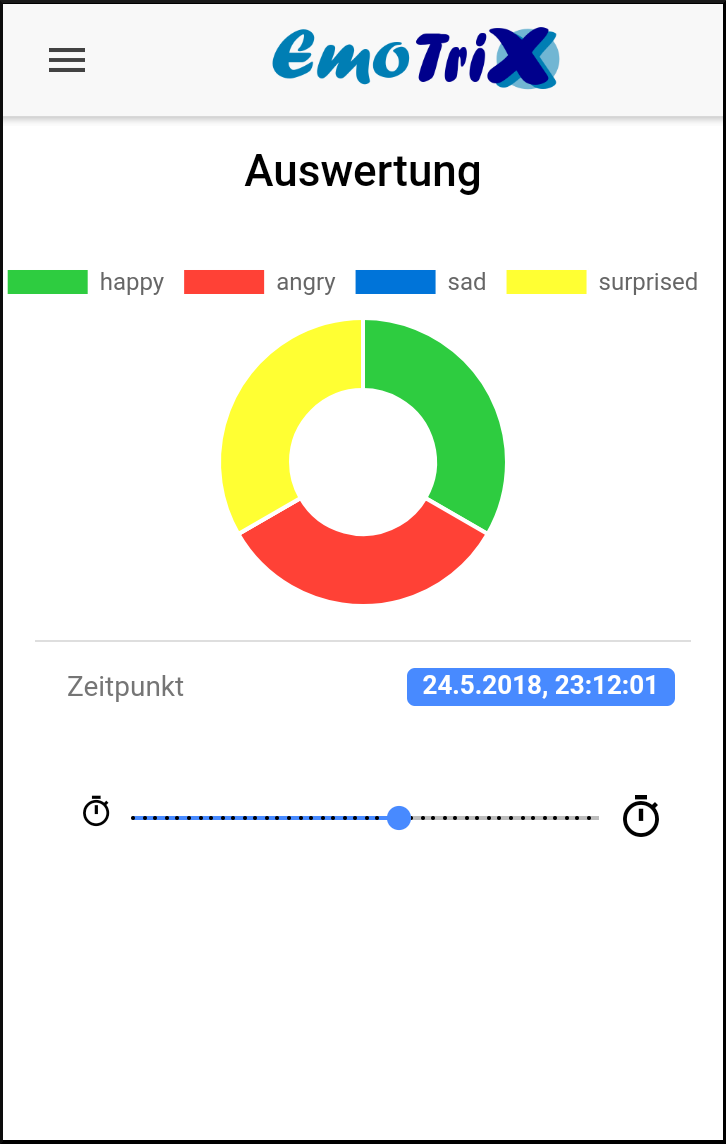
\includegraphics[width=6cm]{Bilder/decisionpage.png}
	\caption[GUI der DecisionPage]{GUI der DecisionPage}
\end{figure}%
\newline
Die Anzeige von EmotionScores erfolgt über ein Pie-Chart, dass die Scores für die Emotionen happy, angry, sad und suprised anzeigt. Die Emotion, die den größten Anteil des Pies hat, ist die Emotion, die der User am wahrscheinlichsten zu diesem Zeitpunkt hatte. Durch klicken auf ein Segment des Pie-Charts wird angezeigt, welchen Score die jeweilige Emotion erreicht hat.\newline
Wie bereits erklärt, erzeugt der Decider in 10-Sekunden-Intervallen für alle in diesem Intervall enthaltenen IndicatorScores eine Menge von EmotionScores. Wenn der User die DecisionPage aufruft, werden ihm die EmotionScores der ersten 10 Sekunden angezeigt. Im blauem Kasten auf der rechten Seite des Bildschirms wird die Startzeit des aktuellen 10-Sekunden-Intervalls angezeigt. Mithilfe des Sliders kann das Intervall verändert werden. Dabei befindet sich ganz links der Zeitpunkt, an dem zum ersten Mal Daten erfasst wurden, wohingegen sich ganz recht der Zeitpunkt det letzten Datenerfassung befindet. In Schritten von 10 Sekunden kann der User mit dem Slider das Intervall auswählen, zu dem die Emotionscores angezeigt werden sollen. Das Pi-Chart wird dementsprechend automatisch angepasst. \newline
Mithilfe der ersten Option des Seitenmenüs kann der User wieder zurück zur HomePage gelangen, um erneut Emotionstest durchzuführen. 
\subsubsection{TutorialPage}
\subsubsectionauthor{Lukas Seemann}
Im Seitenmenü der App befindet sich die Option eine Anleitungsseite aufzurufen. Dieser Screen heißt intern TutorialPage. Da diese Seite sehr simpel aufgebaut ist, ist hiervon kein Screenshot abgebildet. \newline
Auf dieser Seite ist ein Video eingebunden, das durch Anklicken abgespielt werden kann. Das Video ist ein Tutorial, das zeigt wie die Sensoren der App und die einzelnen Emotionstest durchgeführt werden soll und wie die App bedient wird. Das Tutorial-Video bildet zusammen mit dem Kapitel (\textit{Benutzeroberfläche der App}) eine Bedienungsanleitung für die App emoTrix.